	\section{Repérage (12 points)}


\begin{center}
	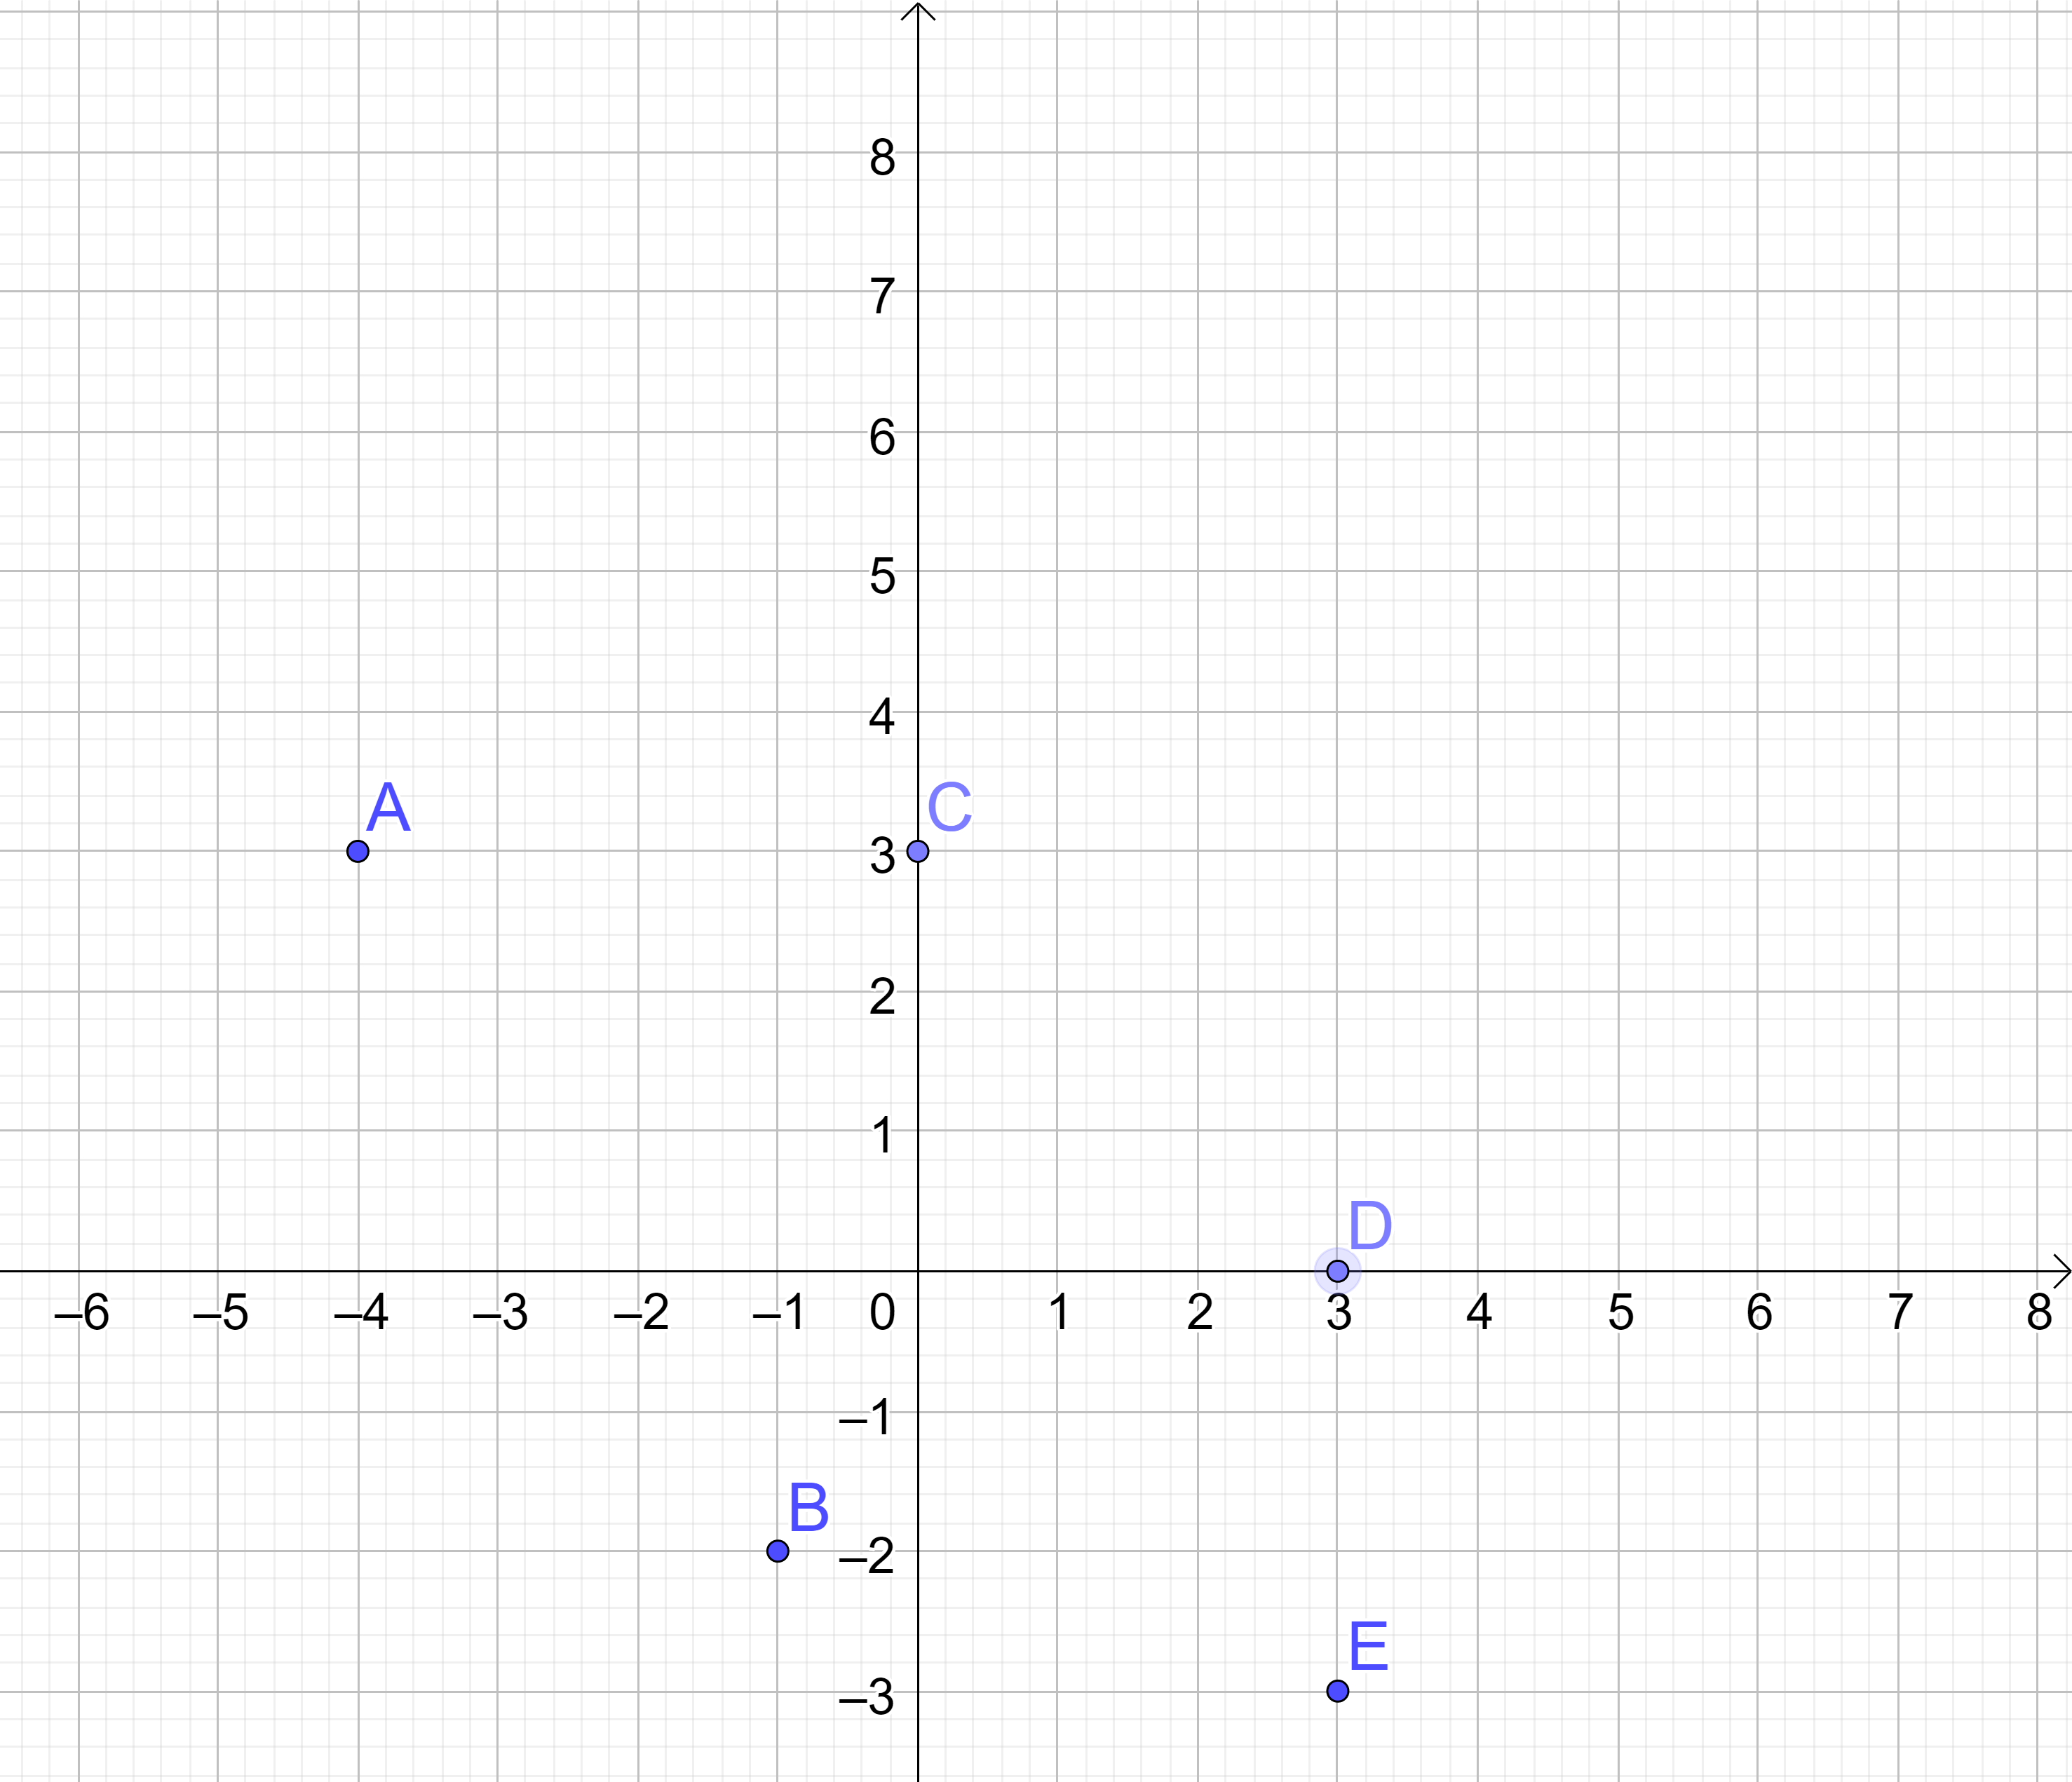
\includegraphics[scale=0.135]{img/grille}
\end{center}

\begin{questions}
	
	\question[5] Donner les coordonnées des 5 points présents dans ce repère.
	\fillwithdottedlines{2cm}
	
	\question[5] Placer les points suivants :
	$F$(+2 ; -1), $G$(-2 ; 0),  $H$(-4 ; -3),  $I$(+5 ; 1 ) et  $J$(0 ; -3)
	
	
	\question[1]  Donner deux points de même abscisse.
	\fillwithdottedlines{1.5cm}
	\begin{solution}
		
	\end{solution}
	
	
	\question[2]  Donner deux points de même ordonnée.
	\fillwithdottedlines{1.5cm}
	\begin{solution}
		
	\end{solution}
	
	
\end{questions}
	
\section{Nombres relatifs (4 points)} 

\begin{questions}
	
	\question[1] Donner deux nombres opposés.
	\fillwithdottedlines{1cm}
	

	\question[1]  Donner deux nombres qui ont le même signe mais pas la même distance à zéro.
	\fillwithdottedlines{1cm}

	\question[1]  Donner deux nombres qui ont la même distance à zéro mais pas le même signe.
	\fillwithdottedlines{1cm}
	
	\question[1]  Donner deux nombres qui n'ont ni la même distance à zéro ni le même signe.
	\fillwithdottedlines{1cm}
\end{questions}



\section{Comparaisons}

Soit les nombres suivants :
$(-2)$; $(-\num{9.384})$; $(-\num{5.63})$; $(+\num{3.5})$; $(+\num{5.3})$ ; $(-\num{3.34})$; $(+\num{9.3})$; $(-\num{7.5})$; $(-\num{5.634})$; $(+\num{7.4}) $; $(+ \num{3.498} ); (+\num{5.347})$ 

\begin{questions}
	\question[1] Quel nombre a la plus grande distance à zéro ?
	\fillwithdottedlines{1cm}
	
	\question[1] Quel nombre a la plus petite distance à zéro ?
	\fillwithdottedlines{1cm}
	
	\question[2] Classer ces nombres par ordre croissant :
	\fillwithdottedlines{2cm}
\end{questions}

